\documentclass[a4paper, 12pt]{article}

\usepackage[T2A]{fontenc}
\usepackage[utf8]{inputenc}
\usepackage[english,russian]{babel}
\usepackage[left=15mm, top=20mm, right=15mm, bottom=20mm, nohead, nofoot]{geometry}

\usepackage{hyperref}
\usepackage{graphicx}
\usepackage{wrapfig}
\usepackage{afterpage}
\usepackage{amsmath, amsfonts, amssymb, amsthm, mathtools}
\author{Хомутов Андрей, группа Б06-903}
\title{ВПВ по курсу "Электричество и магнетизм" \\ Конденсатор на высоких частотах}
\date{22 декабря 2020 г.}
%%%%%%%%%%%%%%%%%%%%%%%%%%%%%%%%%%%%%%%%%%%%%%%%%%%%%%%%%%%%%%%%%%%%%%%%%
\usepackage{graphicx, wrapfig, subcaption, setspace, booktabs}
\usepackage[protrusion=true, expansion=true]{microtype}
\usepackage[english]{babel}
\usepackage{sectsty}
\usepackage{url, lipsum}
\newcommand{\HRule}[1]{\rule{\linewidth}{#1}}
\onehalfspacing
\setcounter{tocdepth}{5}
\setcounter{secnumdepth}{5}
%%%%%%%%%%%%%%%%%%%%%%%%%%%%%%%%%%%%%%%%%%%%%%%%%%%%%%%%%%%%%%%%%%%%%%%%%


\begin{document}

\title{ \normalsize \textsc{Лабораторная работа}
		\\ [4.0cm]
		\HRule{0.5pt} \\ [0.3cm]
		\LARGE \textbf{{Кольца Ньютона}}
		\HRule{0.5pt} \\ [0.1cm]
		\normalsize  \vspace*{18\baselineskip}}

\date{}

\author{%Шамарина Екатерина, Б06-903 \\
		Хомутов Андрей, Б06-903 \\
ФБМФ, 2021\\ }

\maketitle
\thispagestyle{empty}
\newpage
%%%%%%%%%%%%%%%%%%%%%%%%%%%%%%%%%%%%%%%%%%%%%%%%%%%%%%%%%%%%%%%%%%%%%%%%%
\section*{Цели работы} 
Познакомиться с явлением интерференции в тонких плёнках (полосы равной толщины) на примере колец Ньютона и с методикой интерференционных измерений кривизны стеклянной поверхности.
%%%%%%%%%%%%%%%%%%%%%%%%%%%%%%%%%%%%%%%%%%%%%%%%%%%%%%%%%%%%%%%%%%%%%%%%%
 
\section{Теоретическая часть}
%\subsection{...}

%\subsubsection{...}
\begin{wrapfigure}{l}{0.35\linewidth} 
		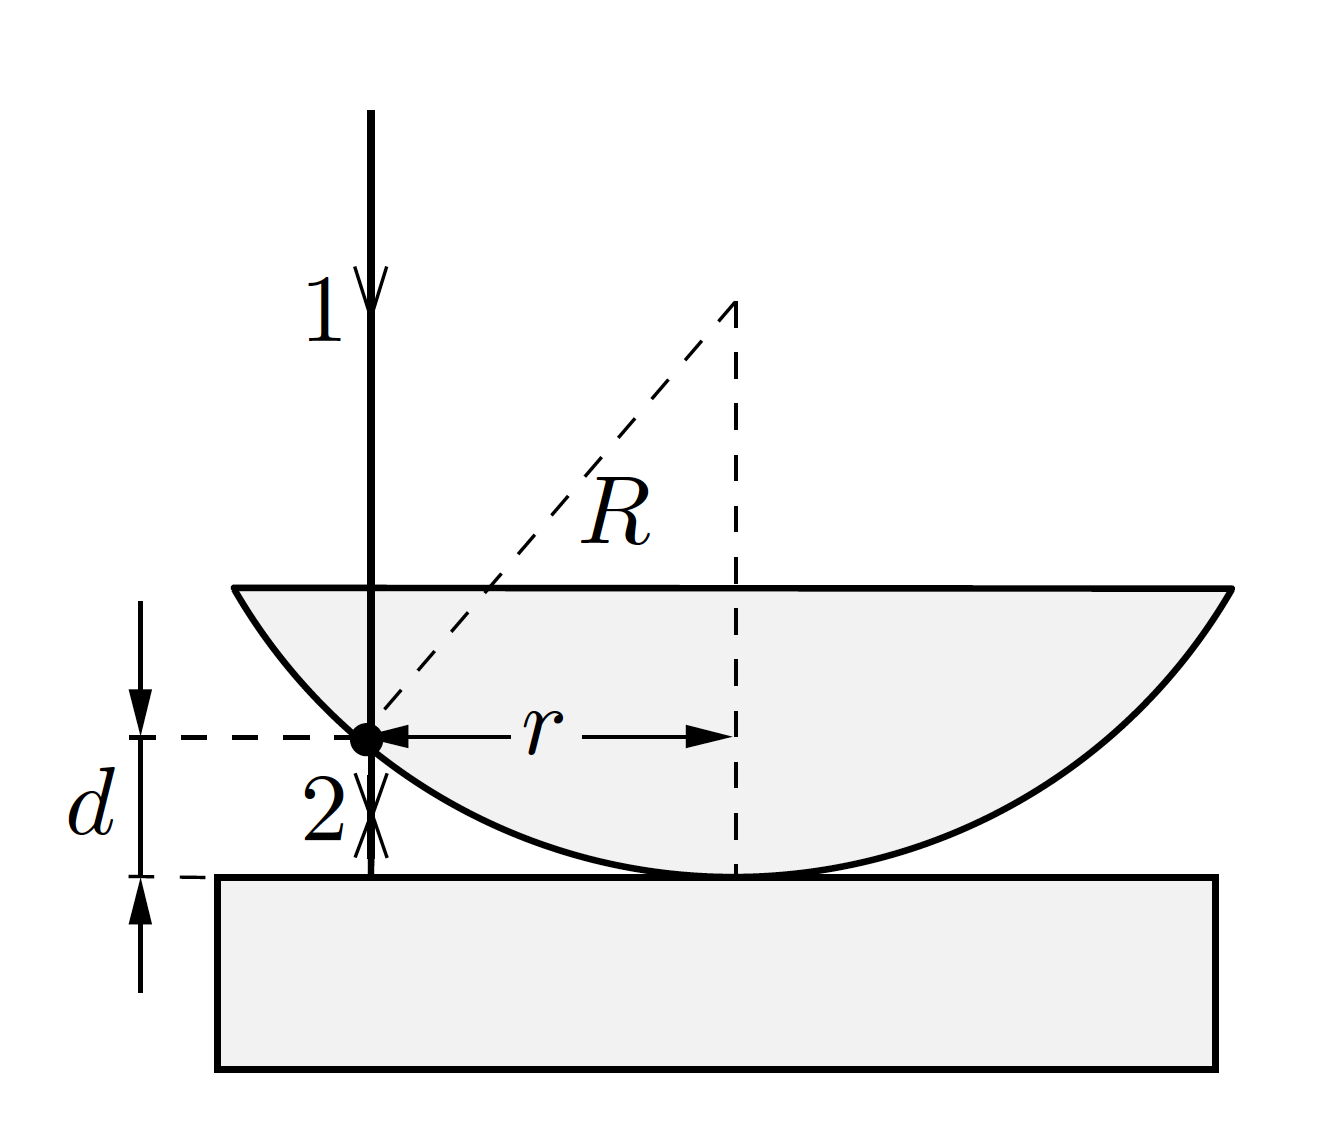
\includegraphics[width=\linewidth]{ring}
		\caption{Ход лучей в линзе}
		\label{ring}
\end{wrapfigure}


Этот классический опыт используется для определения радиуса кривизны сферических поверхностей линз. В этом опыте наблюдается интерференция волн, отражённых от границ тонкой воздушной прослойки, образованной сферической поверхностью линзы и плоской стеклянной пластиной. При нормальном падении света (рис. 1) интерференционные полосы локализованы на сферической поверхности и являются полосами равной толщины.
	
Геометрическая разность хода между интерферирующими лучами равна удвоенной толщине воздушного зазора $ 2d $ в данном месте. Для точки на сферической поверхности, находящейся на расстоянии $ r $ от оси системы, имеем $ r^2 = R^2 - (R - d)^2 = 2Rd - d^2 $, где $ R $ --- радиус кривизны сферической поверхности.
	
При $ R \gg d $ получим$  d = r^2/2R $. С учётом изменения фазы на $ \pi $ при отражении волны от оптически более плотной среды (на границе воздух-стекло) получим \textit{оптическую разность хода интерферирующих лучей}:
	
\begin{equation}\label{r_m}
\Delta = \dfrac{\lambda}{2} + 2d = \dfrac{r^2}{R} + \dfrac{\lambda}{2}
\end{equation}
	
Из условия интерференционного минимума $ \Delta = \dfrac{(2m +1)\lambda}{2}, \; m =0, 1, 2.. $ получим радиусы темных колец $ r_m $:
	
\begin{equation}\label{r_m'}
r_m = \sqrt{m \lambda R}.
\end{equation}

Из аналогичного условия максимума $ \Delta = m \lambda $ радиусы светлых $ r_m' $ 
\begin{equation}\label{r_m'}
r_m' = \sqrt{\dfrac{(2m-1) \lambda R}{2}}.
\end{equation}
\newpage

\section{Практическая часть}
%\subsection{...}
	\begin{wrapfigure}{r}{0.5\linewidth} 
	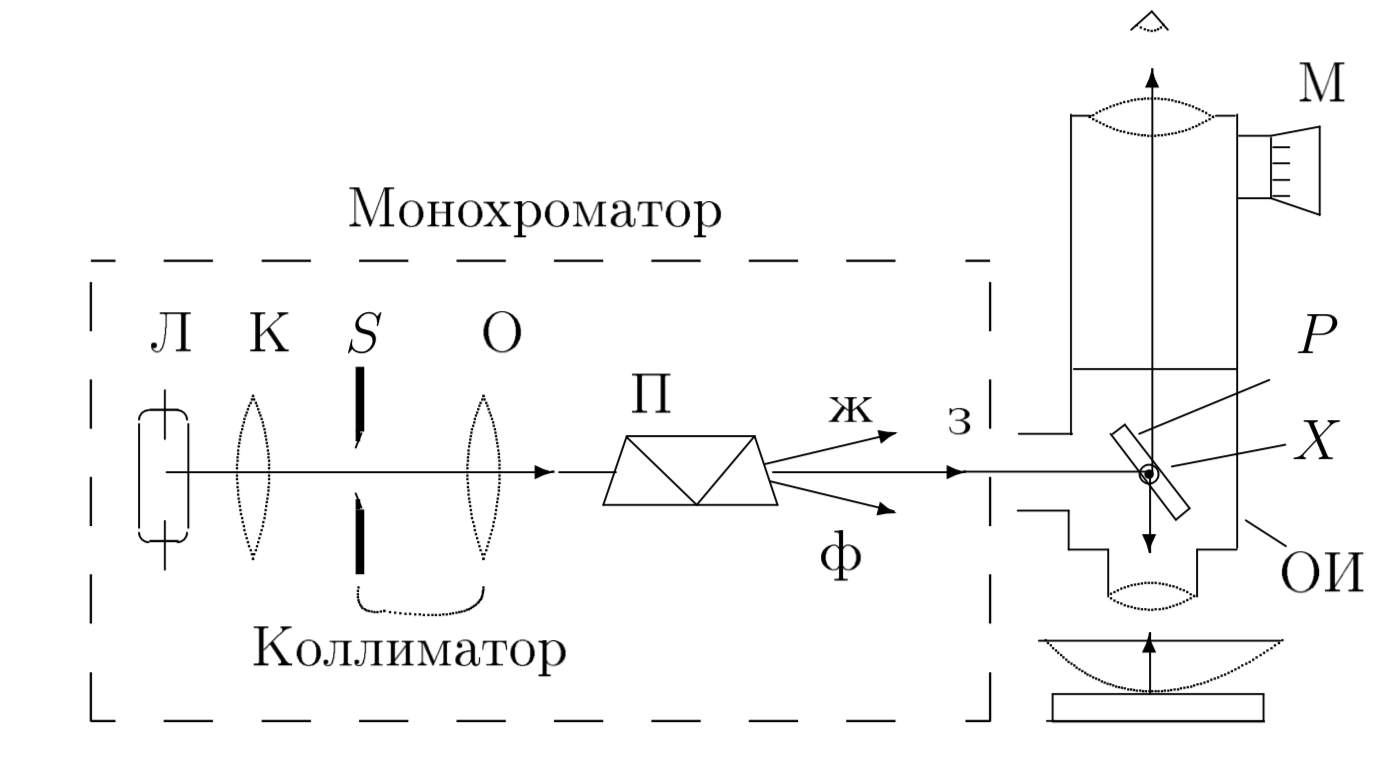
\includegraphics[width=\linewidth]{lab}
	\caption{Экспериментальная установка}
	\label{lab}
\end{wrapfigure}
Были измерены координаты колец слева и справа от центра. Погрешность измерения $\delta_x$ = 2 ед. измерения шкалы (по 1 на погрешность шкалы и "визуальную" ошибку определения положения кольца). Результаты с расчетом квадрата радиуса представлены в таблице 1.



Из формул 2 и 3 следует что по наклону зависимости квдрата радиуса колец от их номера (рис. 3) можно определить радиус кривизны линзы $R = \frac{k}{ \lambda}$. Учитывая $\lambda_g$ = 546 нм, получаем R = 1.45$\pm$0.14 см.

\begin{table}[h!]
\begin{center}
\caption{Радиусы колец Ньютона}
\begin{tabular}{|c|c|c|c|c|c|c|c|c|}
\hline
\multicolumn{1}{|l|}{} & \multicolumn{3}{c|}{Темные кольца}         &                                   & \multicolumn{4}{c|}{Светлые кольца}                                          \\ \hline
№                      & x1, мм & x2, мм & $r^2 \cdot 10^3$, мм$^2$ & $\delta_{r^2} \cdot 10^3$, мм$^2$ & x1    & x2    & $r'^2 \cdot 10^3$, мм$^2$ & $\delta_{r'^2} \cdot 10^3$, мм$^2$ \\ \hline
0                      & 0,36   & 0,445  & 1,81                     & 0,04                              & -     & -     & -                        & -                                 \\ \hline
1                      & 0,318  & 0,496  & 7,92                     & 0,16                              & 0,342 & 0,473 & 4,29                     & 0,09                              \\ \hline
2                      & 0,281  & 0,533  & 15,9                     & 0,3                               & 0,3   & 0,516 & 11,66                    & 0,25                              \\ \hline
3                      & 0,248  & 0,561  & 24,5                     & 0,6                               & 0,266 & 0,547 & 19,7                     & 0,4                               \\ \hline
4                      & 0,227  & 0,587  & 32,4                     & 0,8                               & 0,239 & 0,573 & 27,9                     & 0,7                               \\ \hline
5                      & 0,206  & 0,606  & 40,0                     & 1,0                               & 0,217 & 0,597 & 36,1                     & 0,9                               \\ \hline
6                      & 0,187  & 0,625  & 48,0                     & 1,3                               & 0,201 & 0,614 & 42,6                     & 1,1                               \\ \hline
7                      & 0,168  & 0,641  & 55,9                     & 1,7                               & 0,178 & 0,633 & 51,8                     & 1,5                               \\ \hline
8                      & 0,15   & 0,656  & 64,0                     & 2,1                               & 0,16  & 0,649 & 59,8                     & 1,9                               \\ \hline
9                      & 0,136  & 0,674  & 72,4                     & 2,6                               & 0,143 & 0,666 & 68,4                     & 2,3                               \\ \hline
10                     & 0,123  & 0,688  & 80                       & 3                                 & 0,129 & 0,68  & 75,9                     & 2,8                               \\ \hline
\end{tabular}
\end{center}
\end{table}



Освещая установку зеленым и желтым светом ($\lambda_y$ = 578 нм) можно было наблюдать периодическое ухуджешие видимости интерференционный картины (биения). Между двумя соседними центрами четких систем уложилось $ \Delta m =  19 $ колец. Таким образом, разность длин волн можно расчитать как:
$$
	(\Delta m + 1)\lambda_g = \Delta m \lambda_y => \Delta \lambda = \dfrac{\lambda_g}{\Delta m} \simeq 29\text{ нм}.
$$

\newpage
\begin{figure}[h!]
    \begin{center}
    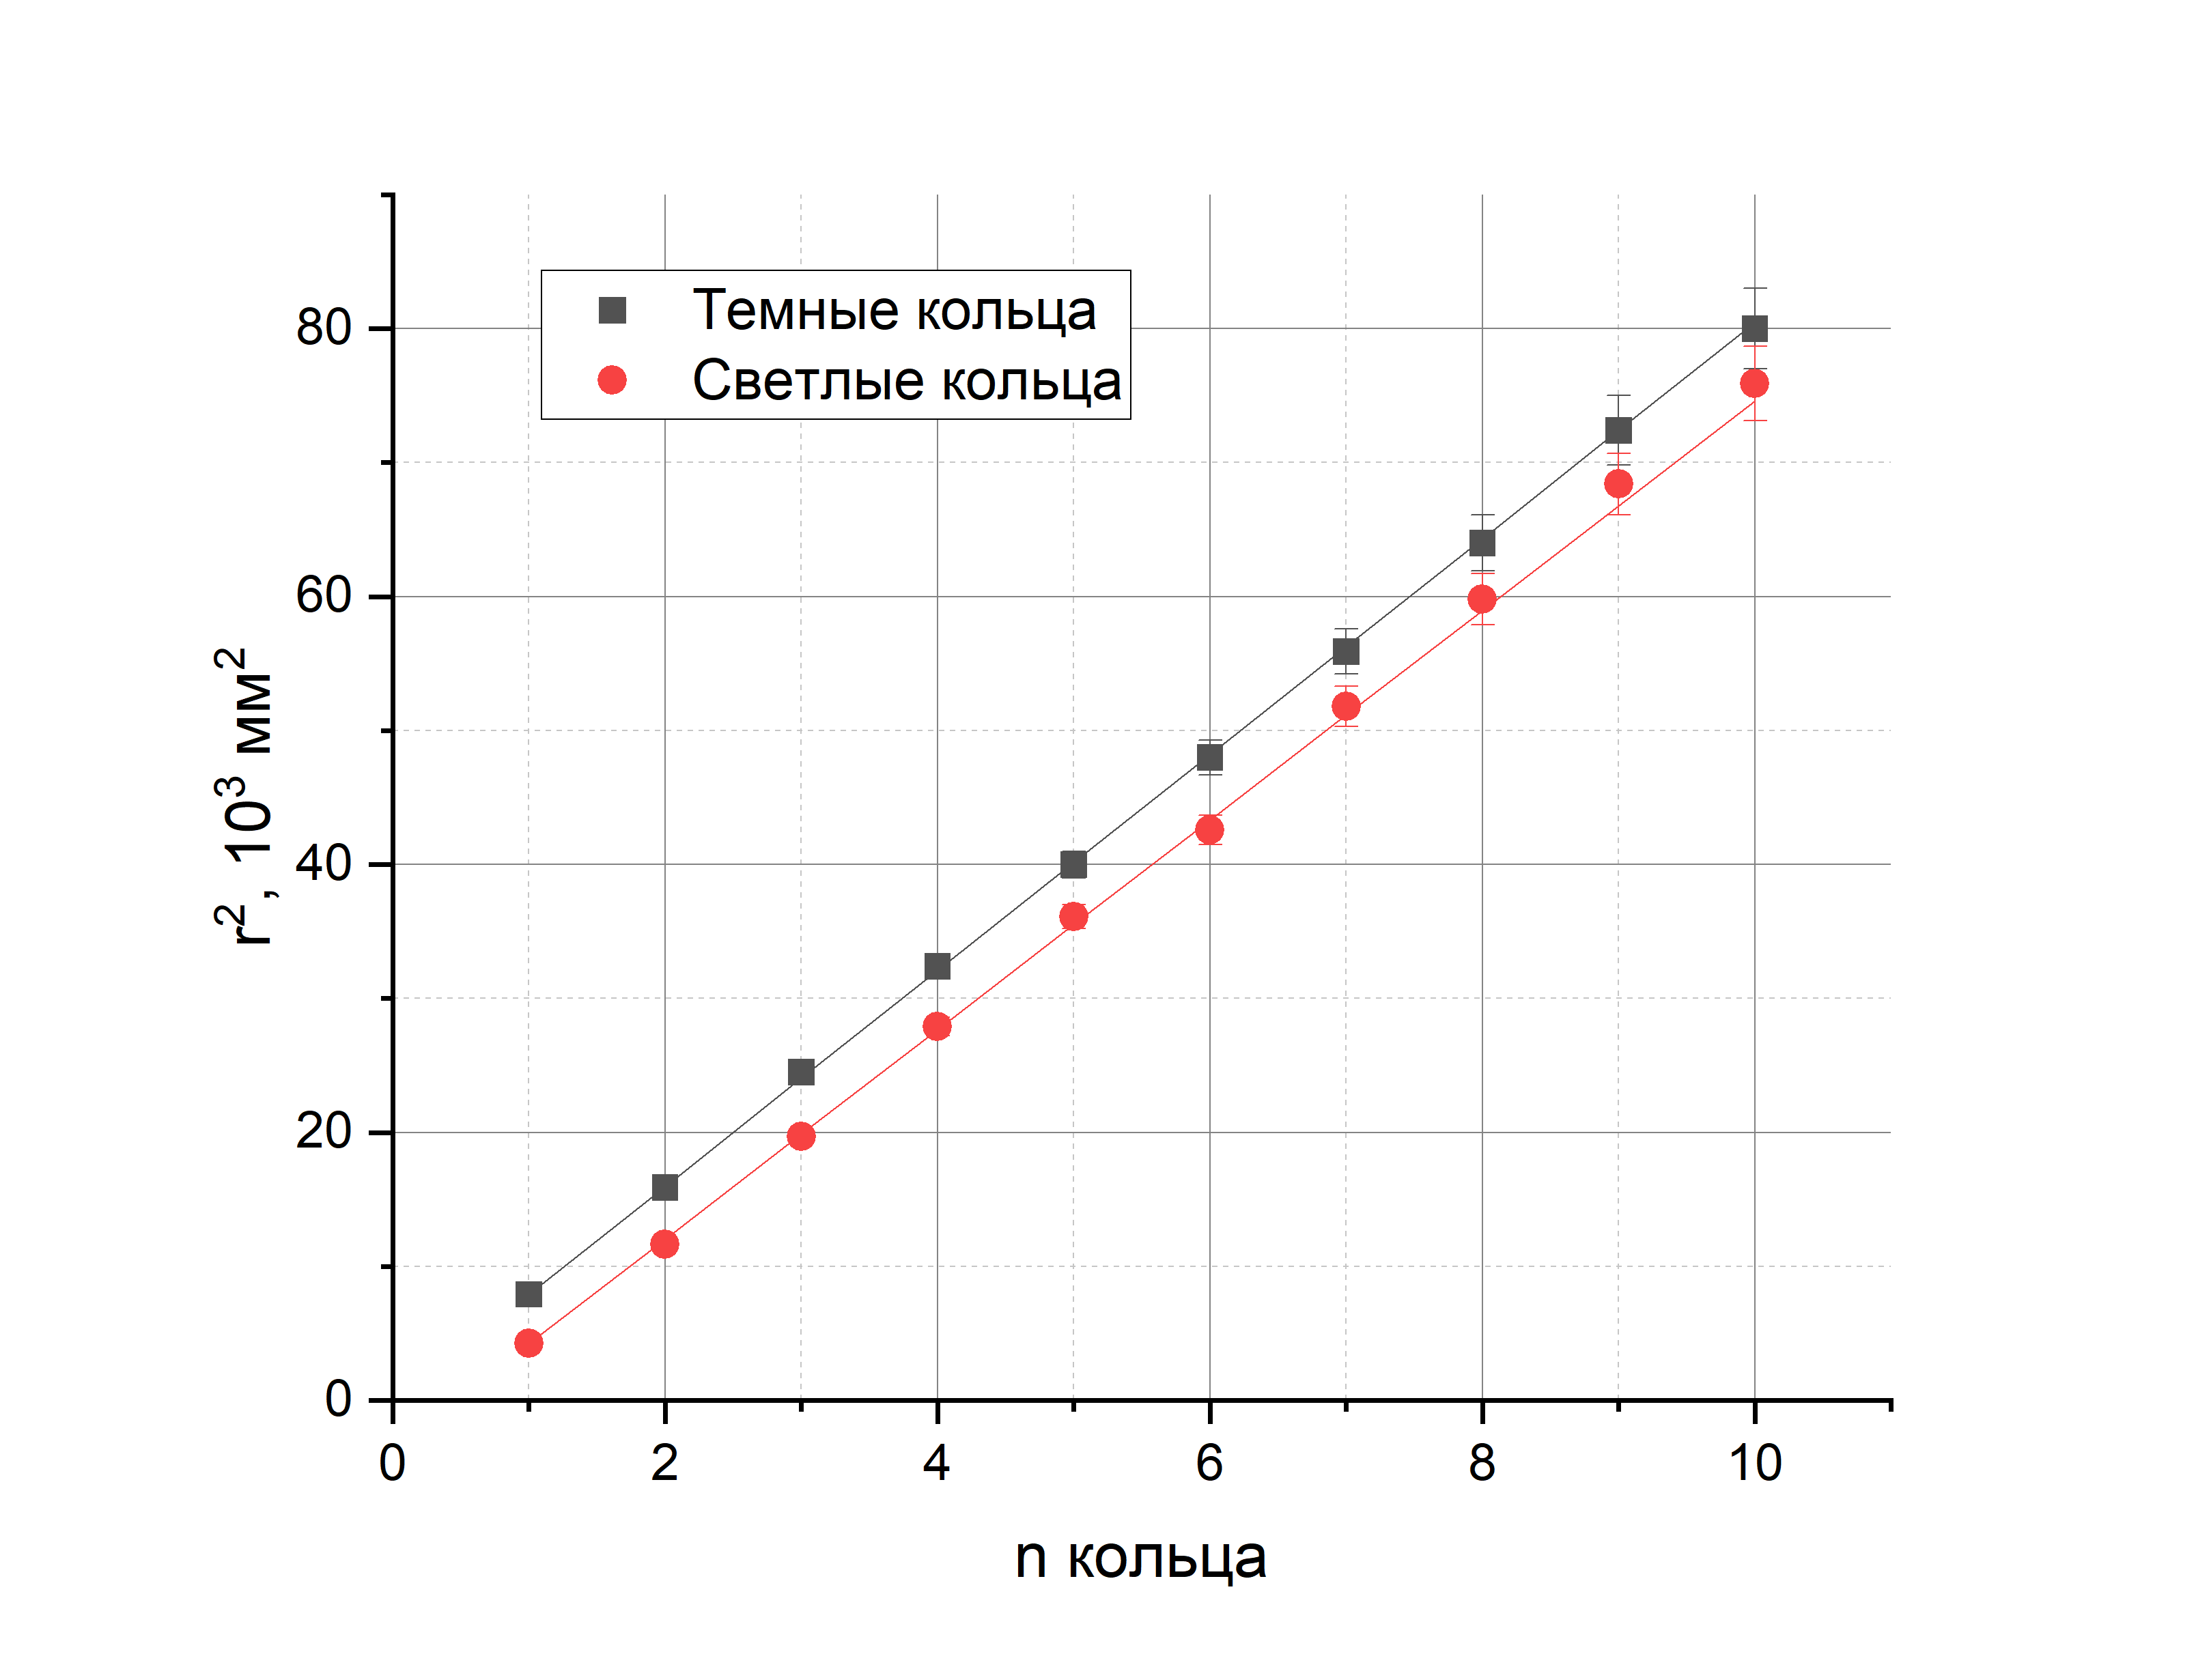
\includegraphics[width=1\textwidth]{graph1.png}
    \end{center}
    \caption{Зависимоть квадрата радиуса от номера кольца}
\end{figure}

%%%%%%%%%%%%%%%%%%%%%%%%%%%%%%%%%%%%%%%%%%%%%%%%%%%%%%%%%%%%%%%%%%%%%%%%%

 \section{Выводы}
\begin{enumerate}
    \item Была получена интерференционная картина колец Ньютона. По зависимости радиуса колец от их номера был вычислен радиус кривизны линзы из установки
    \item Были получены биения. По периоду изменения видности была оценена разность длин волн, получившееся равно 29 нм. Одидаемая - 32 нм.

\end{enumerate}

\end{document}


\begin{figure}[h!] %% ШАБЛОН ДЛЯ ДВУХ КАРТИНОК
\begin{center}
\begin{minipage}[h]{0.40\linewidth}
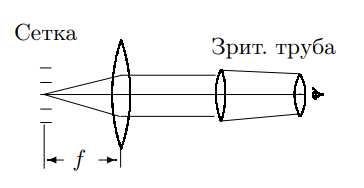
\includegraphics[width=1\linewidth]{plus_lens.PNG}
\caption{...} %% подпись к рисунку
\label{ris:experimoriginal} %% метка рисунка для ссылки на него
\end{minipage}
\hfill 
\begin{minipage}[h]{0.40\linewidth}
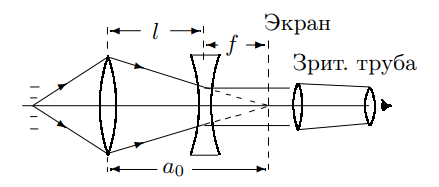
\includegraphics[width=1\linewidth]{minus_lens.PNG}
\caption{..}
\label{ris:experimcoded}
\end{minipage}
\end{center}
\end{figure}